\section{Objectives} \label{chapter3:objectives}
\nt{TODO title not clear enough}

\illustration{state of the art schema step 5}

% The objective of this thesis is to find a reconciliation of the two goals, by finding an equivalence between two approaches with different goals, in the case of streaming web applications.

The section \ref{chapter3:software-design} shows modularity is the best organization to improve maintainability of an application.
This organization is best supported by a functional approach.
Indeed, higher-order programming improves readability and maintainability.
However, higher-order programming, and modular programming in general, requires the use of a global memory store.

The section \ref{chapter3:software-efficiency} shows that to attain scalability, an application needs to be organized to distribute its memory store into independent silos to multiply the exclusive accesses.
Still, many works provide this global memory store interface to developers, because it is the best way to support the modularity advocated in section \ref{chapter3:software-design}.
This incompatibility between these two organization, and their goals is responsible for the shifts operated during the life of an application.
Huge developing efforts are made to translate manually from one organization into the other, and to maintain the implementation despites its unmaintainable nature.
% when the most pressing need shift from maintainability to performance, or vice versa.

In section \ref{chapter3:reconciliations}, we show different tentatives to reconciles the two organizations.
Most are satisfactory for specific domains, such as the high-performance computing.
It is profitable, as the expected speedup of developing an application with an adapted programming model compensates the huge development effort.
%  where it is accepted to spend long time developing an application to use thousands of accelerators to compute heavy calculation, because the expected speedup is profitable, compared to develop an application for all these thousands accelerators.
However, none are satisfactory in the case of web applications because the need for performance is always uncertain.
The development effort is not required at the beginning, hence its cost cannot be justified.
It is only when the audience increases, often with the revenue, that the cost for the development effort can be justified.
This situation illustrate the need for a programming model reconciling the two concerns, of maintainability and performance.
% Indeed, they all are too specific, and require too much from the developer to be accepted at a large scale.

% \comment{Here a table summarizing the different approaches, and the sweet spot.}

\begin{table}
\begin{tabular}{l|l|l|l}
             & Maintainability         & Performance           & Both\\\hline
General      & Functional Programming  & Message-passing       & Loop parallelization\\
Web          & Javascript              & Pipeline architecture & ø
\end{tabular}
\caption{Summary of the state of the art}
\label{tab:chapter3:objectives:summary}
\end{table}

Our objectives is to find an equivalence between these two organization, specifically for the case of web applications.
To do so, we focus on the Javascript programming language, and specifically, the node.js interpreter.
As explained in the end of chapter \ref{chapter2}, the execution model of Javascript is similar to a pipeline.
We intend to split a node.js application into a parallel pipeline of stages.

The contribution of this thesis is organized in two chapters, as illustrated in figure \ref{fig:chapter3:objectives:roadmap}.
In chapter \ref{chapter4} I present the extraction of a pipeline of operations from a Javascript application.
I show that such pipeline is similar to the one exposed by Promises, and I propose a simpler alternative to the latter called Dues.
However, these operations still require a global memory for coordination so they are not executed in parallel.
In chapter \ref{chapter5}, we present the isolation of the operations into isolated containers called Fluxions. 

\begin{figure}[h!]
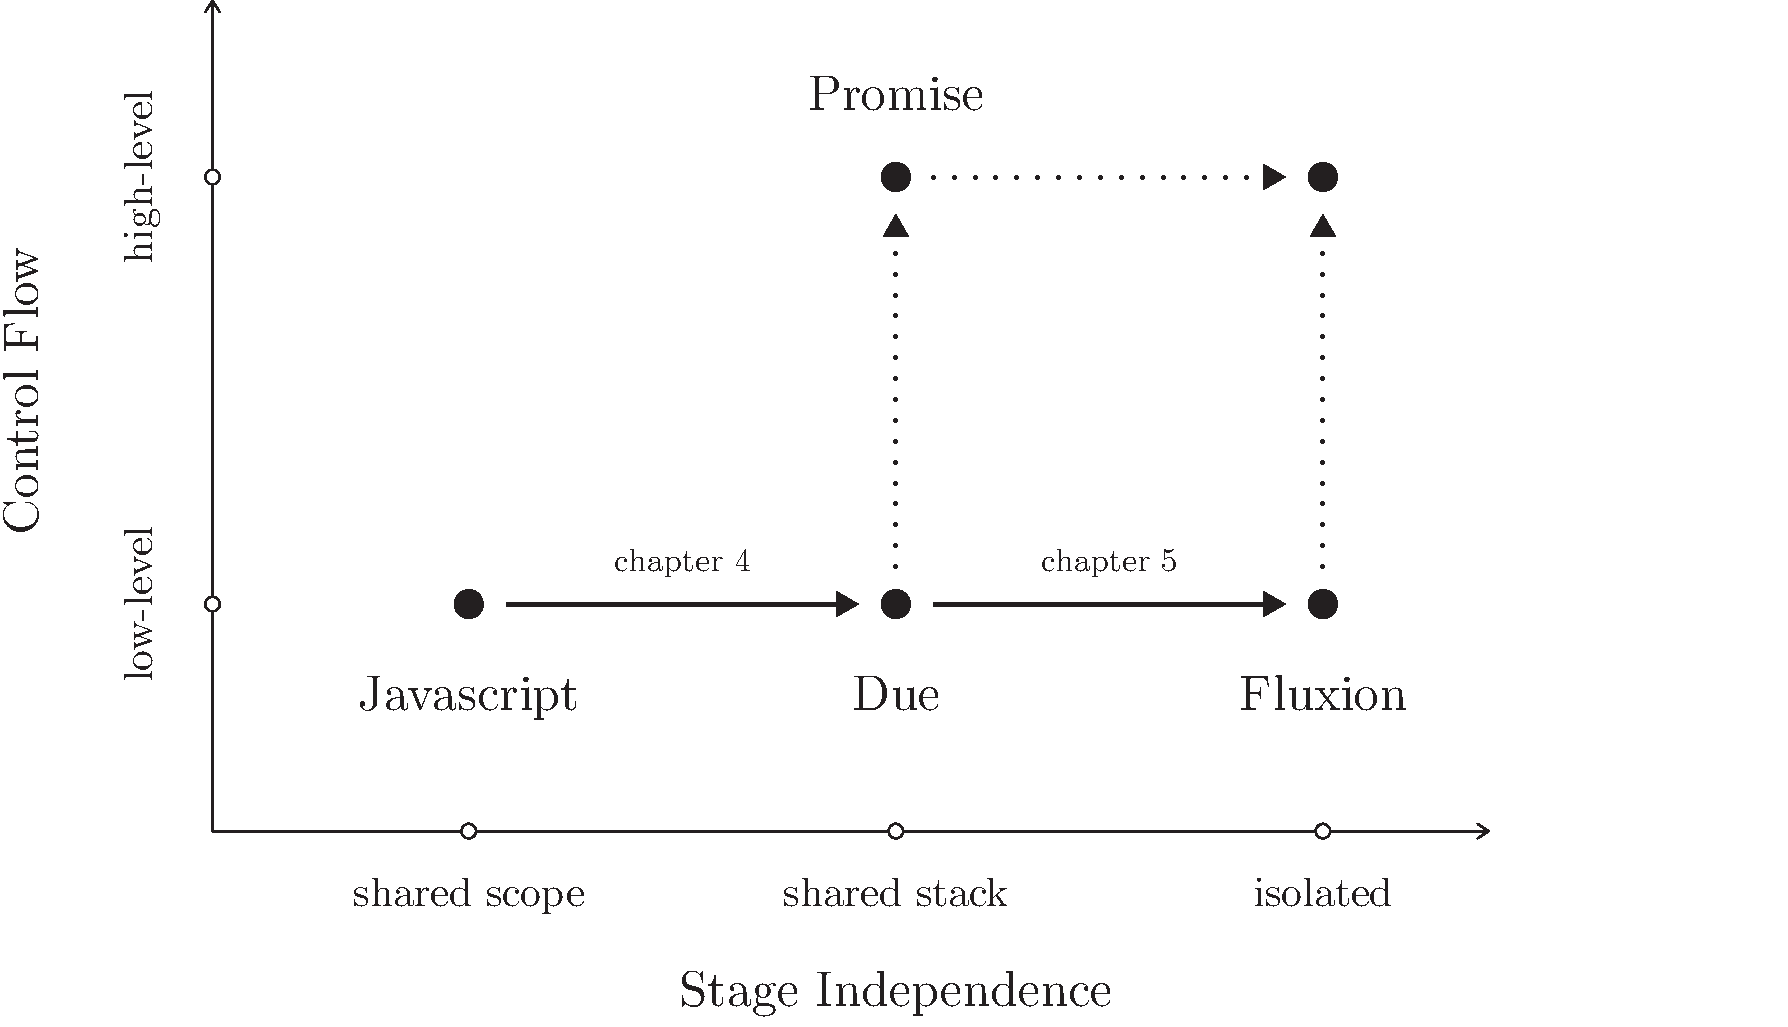
\includegraphics[width=1\textwidth]{../ressources/roadmap.pdf}
\caption{Roadmap for this work}
\label{fig:chapter3:objectives:roadmap}
\end{figure}

\begin{center}
\rule{3cm}{0.4pt}
need integration
\rule{3cm}{0.4pt}
\end{center}

We show that there is no languages that features higher-order functions to improve modularity, a common memory store easy to develop with, but at the same time provides scalable concurrency.

We aim at filling this gap, and for a concrete example, focus our work on the Javascript programing language.
Indeed, Javascript features higher-order functions, is highly-used in concurrent context, but lacks scalable concurrency.








\subsection{Equivalence}

\subsubsection{Rupture Point}

The execution of the pipeline architecture is well delimited in isolated stages.
Each stage has its own thread of execution, and is independent from the others.
On the contrary, the code of the event-loop is linear because of the continuation passing style and the common memory store.
% The message passing linking the callbacks is transparently handled by the event-loop.
However, the execution of the different callbacks are as distinct as the execution of the different stages of a pipeline.
The call stacks of two callbacks are distincts.
Therefore, an asynchronous function call represents the rupture between two call stacks.
It is a rupture point, and is equivalent to a data stream between two stages in the pipeline architecture.

Both the pipeline architecture and the event-loop present these rupture points.
The detection of rupture points allows to map a pipeline architecture onto the implementation following the event-loop model.
To allow the transformation from one to the other, this thesis studies the possibility to detect rupture points, and to distribute the global memory into the parts defined by these rupture points.
The detection of rupture points is addressed in chapter \ref{chapter4}.

\subsubsection{Invariance}

% This transformation is important on two points.
% The conservation of the invariance.
% The equivalence between the coordinations.

The transformation should preserve the invariance as expressed by the developer to assure the correctness of the execution.
The partial ordering of events in a system, by opposition to total ordering, is sufficient to assure this correctness.
% This result was used by Lamport to prove the correctness of distributed systems.
The global memory is a way to assure the total ordering of events, and the message passing coordination is a way to assure partial ordering of events.
Therefore, to assure the correctness of the execution of a system, the state coordination with a global memory is equivalent to message passing coordination.
And it is possible, at least for some rupture points, to transform the global memory coordination into message passing while conserving the correctness of execution.

In order to preserve the invariance assured by the event-loop model after the transformation, each stage of the pipeline needs to have an exclusive access to memory.
The global memory needs not to be split into parts and distributed into each of the stages.
To assure the missing coordinations assured by the shared memory between the stages, the transformation should provide equivalent coordination with message passing.
The isolation and replacement of the global memory is fully address in chapter \ref{chapter5}

% The invariance holds for the whole memory during the execution of each callback.
% As I explained in the previous section, this invariance is required to allow the concurrent execution of the different tasks.
% On the other hand, the invariance is explicit in the pipeline architecture, as all the stages have isolated memories.
% The coordination between these isolated process is made explicit by the developer through message passing.

% I argue that the state coordination between the callbacks requireing a global memory could be replaced by the message passing coordination used manually in the pipeline architecture.
% I argue that not all applications need concurrent access on the state, and therefore, need a shared memory.
% % Specifically, I argue that each state region remains roughly local to a stage during its modification.
% \nt{TODO review that, I don't know how to formulate these paragraphs. Identify the state and the data in the global memory.}

% \subsubsection{Transformation}

% This equivalence should allow the transformation of an event loop into several parallel processes communicating by messages.
% In this thesis, I study the static transformation of a program, but the equivalence should also hold for a dynamic transformation.
% I present the analyzis tools I developed to identify the state and the data from the global memory.
